\section{Lecture 7: Reconstructor: Ideal and practical}


\subsection{Introduction}
In the previous lecture, we saw that a band-limited signal can be perfectly reconstructed from its samples, if it has been sampled at a frequency greater than twice the maximum frequency of the original signal $f_{m}$. In this lecture we will see what the procedure for reconstruction is by analysing in the frequency domain. 


\subsection{Frequency response for Ideal filter for reconstruction}
It was shown that sampling creates multiple copies of the original spectrum shifted by integer multiples of the sampling frequency $f_{s}$. In order to fully reconstruct the original signal, we need a system which retains the original spectrum and cuts-off the copies as shown in Fig.\ref{copies}.

\begin{figure}[h] 
        \centering
                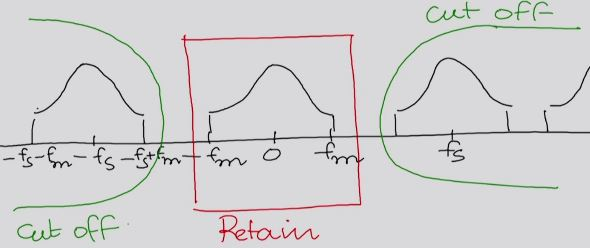
\includegraphics[width=0.8\textwidth]{aliasing.JPG}
                \caption{Principle of reconstruction}
                \label{copies}
\end{figure}

We can achieve this by passing the sampled signal to a LSI system with a frequency response $H(f)$ as shown in Fig.\ref{freq_response}. The filter needs to leave the signal unchanged in the frequency range $-f_{m} - \delta$ to $f_{m} + \delta$ and cut off the rest of the frequencies. 
\begin{figure}[h] 
        \centering
                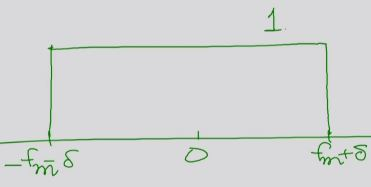
\includegraphics[width=0.8\textwidth]{freq_response.JPG}
                \caption{Desired frequency response of filter}
                \label{freq_response}
\end{figure}
In order to ensure that the copies are completely outside this window, we require $f_{m} + \delta < f_{s} - f_{m}$. This is because from Fig.\ref{copies}, it can be seen that there is a margin between $f_{m}$ and $f_{s} - f_{m}$. As long as the edge of the window falls inside this margin, we are good to go. 

But why do we require this margin? Why do we need to sample at \textit{greater} than twice $f_{m}$? This is because it would create a problem if our signal had a pure sinusoid exactly at $f_{m}$ i.e a \textit{tonal} component. A pure sinusoid of frequency $f_{m}$ in the time domain (a tonal component at $f_{m}$) would imply an impulse at $f = f_{m}$ in the frequency domain. Let us consider such a tonal component and see what happens if we were to sample it exactly at twice its frequency, $f_{s} = 2f_{m}$. This means that we have two samples in every period. In the unlucky event that we sampled at the zero-crossing of the sinusoid, all our samples will simply have a value $0$ as shown in green in Fig.\ref{exact_2}. 
\begin{figure}[h] 
        \centering
                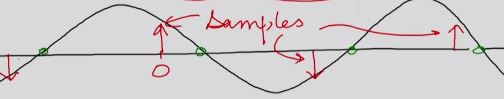
\includegraphics[width=0.8\textwidth]{exact_2.JPG}
                \caption{Sampling at exactly twice $f_{m}$ may yield all samples to be zero}
                \label{exact_2}
\end{figure}

Additionally, the filter should have a cut-off frequency beyond $f_{m}$ as we want to retain the tonal component at $f_{m}$. Hence the margin is necessary. 

\subsection{Impulse response of ideal filter for reconstruction}
To find this, we have to compute the inverse Fourier transform of the filter shown in Fig.\ref{freq_response}. 
\begin{equation} \label{deriv}
\begin{split}
h(t)   & = \int_{-\infty}^{\infty} H(f)e^{j2\pi ft}df \\
& = \int_{-f_{m}-\delta}^{f_{m}+\delta} 1. e^{j2\pi ft}df \\
& = \frac{e^{j2\pi ft}}{j2\pi t} \rvert_{-f_{m}-\delta}^{f_{m}+\delta} \\
& = \frac{e^{j2\pi ft}}{j2\pi t} \rvert_{-f_{c}}^{f_{c}}  \mbox{ where } f_{c} = f_{m} + \delta \\
& = \frac{e^{j2\pi f_{c}t} - e^{-j2\pi f_{c}t}}{j2\pi t} \\
& = \frac{2j\sin (2\pi f_{c}t)}{j2\pi t} 
\end{split}
\end{equation}

The impulse response is basically a \textit{sinc} function. It goes to zero at all integer values of the argument, i.e when $2f_{c}t$ is an integer. 

\subsection{Problems with the ideal reconstructor}
\subsubsection{Stability}
Is the system given by the impulse response $h(t)$ as in \eqref{deriv} a stable system? It can be proven that it is not. For stability we require,
\begin{equation} \label{unstable}
\int_{-\infty}^{\infty} |h(t)|dt < \infty
\end{equation}
\textbf{Challenge} : Show that the above inequality does not hold. In other words, show that the absolute integral of $h(t)$ diverges thereby rendering the system unstable. \\
\textbf{Hint} : Split the integral into pieces. Find some quantity which is smaller than these pieces. Then show that the sum of the smaller quantity diverges meaning that the sum of the actual pieces will definitely diverge. $h(t)$ looks as in Fig.\ref{impulseRes}.
\begin{figure}[h] 
	        \centering
	        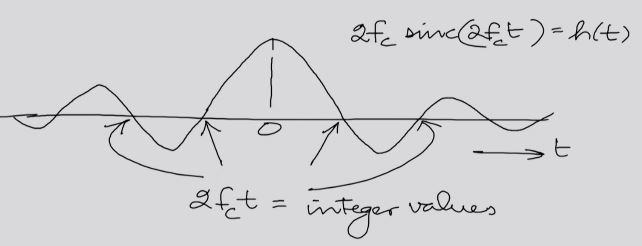
\includegraphics[width=0.8\textwidth]{sinc.JPG}
	                \caption{Impulse response $h(t)$}
	                \label{impulseRes}
\end{figure}
In $|h(t)|$, the negative parts get reflected about the $x$-axis and become positive. \\
Step 1 : Take each of the segments or lobes. \\
Step 2 : Lower bound each of these areas. \\
Step 3 : Show that the sum of these lower-bound areas is itself divergent.\\
\textbf{Note} :  This kind of a frequency response is called as a \textit{brick wall} response because of its structure. Brick-wall responses are always unstable systems. However although this system is unstable, its impulse response has a Fourier transform. In general this need not be the case. It means that if we give this system an input of a sinusoid, we are guaranteed a sinusoid output but there may very well be some bounded inputs whose outputs turn out to be unbounded. Hence while trying to reconstruct a bounded sampled signal, we may end up with an unbounded output if we were to use this filter.\\
What can we do about it? Recall the margin in the frequency response that we asked for earlier. We can make use of this to create a filter which is not brick wall-like and stable. Consider the frequency response of sampled signal (only with frequency values shown) as in Fig. \ref{margin}. 
\begin{figure}[h] 
        \centering
        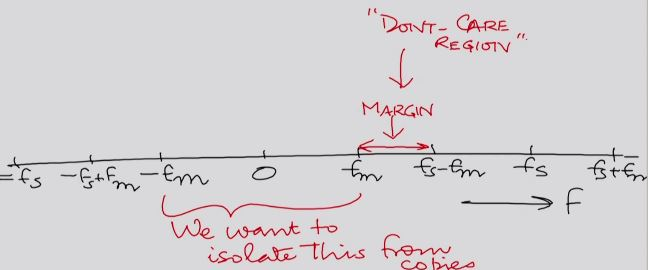
\includegraphics[width=0.8\textwidth]{margin.JPG}
        \caption{Making use of the margin or the \textit{don't care region} to construct a stable filter}
        \label{margin}
\end{figure}
As there is no frequency present in the margin, we do not really care what the filter does to those frequencies, or in other words, the frequency response at those frequencies is immaterial. Using this fact, we can use a filter which is not brickwall-like as in Fig.\ref{not_brick}, for example. 
\begin{figure}[h]
        \centering
                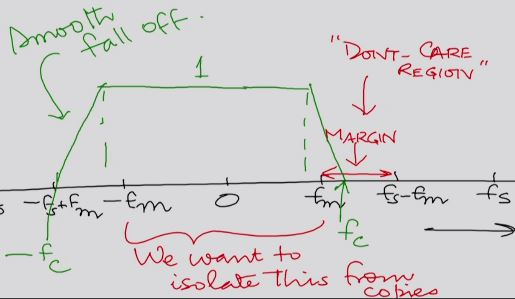
\includegraphics[width=0.8\textwidth]{not_brick.JPG}
                \caption{Example of a filter which is not brickwall-like, but still serves our purpose}
                \label{not_brick}
\end{figure}
This kind of a filter has a frequency response which is \textit{continuous}, unlike the brickwall filter (which had a discontinuity at $f = f_{c}$). So the margin has allowed us to make a stable filter. How large can the margin be? It is governed by the difference between $f_{s}$ and $2f_{m}$. 
\newpage
\subsubsection{Realisability}
Look at both the brickwall filter and the modified stable filter which was continuous. Both have a flat region between $-f_{m}$ and $f_{m}$. It is impossible to realise this practically. The flat region in the frequency response brings in \textit{irrationality} into the response and irrational systems require infinite resources to realise. 

We can make things more practical. Let us try to make a filter which varies \textit{slowly} in the previously flat region. Beyond this region it can be allowed to vary fast (Fig. \ref{vary}).
\begin{figure}[h] 
        \centering
        
                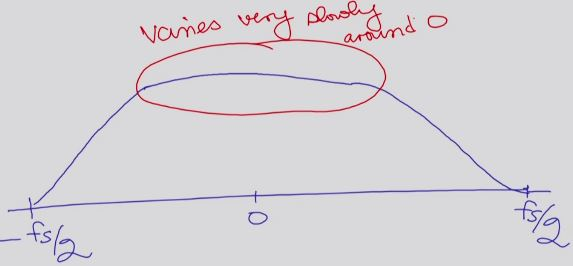
\includegraphics[width=0.8\textwidth]{vary.JPG}
                \caption{A filter which is practically realisable}
                \label{vary}
        
\end{figure}

